%%%--------------------------------%%%
%%% Theory
%%%--------------------------------%%%
\newpage
\section{Gamification}
\label{sec:theoryB}

The following chapter's aim is to clarify the main theory behind human motivation, gamification and the corresponding patterns and methods. Therefore, first of all the term Gamification is defined and explained (chapter \ref{sec:theoryBa}), furthermore there is an introduction to human motivation (chapter \ref{sec:theoryBb}) and motivational design patterns (chapter \ref{sec:theoryBc}). Moreover, the Gamification Design Process is introduced (chapter \ref{sec:theoryBd}). Finally the effectiveness of gamification in terms of business software is discussed. (chapter \ref{sec:theoryBe}).


\subsection{Definition}
\label{sec:theoryBa}

The term gamification is defined by Kumar and Herger as follows:

\begin{fquote}[Gamification {\protect\cite[p. 8]{kumarGamificationWorkDesigning2013}}]
	Gamification is the application of game design principles and mechanics to
	non-game environments. It attempts to make technology more inviting by encouraging users to engage in desired behaviors and by showing the path to mastery.
	From a business viewpoint, gamification is using people’s innate enjoyment of play.
\end{fquote}

Based on the definition above gamification aims to motivate the user to do something \cite[p. 8]{kumarGamificationWorkDesigning2013}. That is why the next chapter provides a more comprehensive introduction on motivation. 


\subsection{Human Motivation}
\label{sec:theoryBb}

The game design principles and mechanics which are used in the context of gamification are a specialization of motivational design patterns used in Human Computer Interaction. \cite[p. 59]{kumarGamificationWorkDesigning2013}

Therefore, this chapter provides an introduction to the three fundamentals of gamification: psychology of motivation, behavioral psychology and behavioral economics - all of them dealing with human motivation.

\paragraph*{Psychology of motivation}
Human motivation is one of the main topics of psychology. Some questions which arise are: What motivates human action? What intentions do they pursue with their doing? Which activities provide pleasure or satisfaction? \cite[p. 1]{bierhoffeditorEnzyklopaediePsychologieSoziale2016}

There are two types of motivation: extrinsic and intrinsic motivation. 
On the one hand, intrinsic motivation is based on an internal drive to do something. Humans are doing this task on their own. Possible motivational factors are gained autonomy, mastery or freedom. \cite[p. 2, 3, 4]{bierhoffeditorEnzyklopaediePsychologieSoziale2016}, \cite[p. 60, 61]{kumarGamificationWorkDesigning2013} Deci describes intrinsic motivation as follows: "One is said to be intrinsically motivated to perform an activity when he receives no apparent rewards except the activity itself." \cite[p. 105]{deciEffectsExternallyMediated1971}

On the other hand, extrinsic motivation is based on motivational factors from the outside, such as money, throphys or the comparison with others (for example with points, levels or leaderboards). \cite[p. 2, 3, 4]{bierhoffeditorEnzyklopaediePsychologieSoziale2016}, \cite[p. 60, 61]{kumarGamificationWorkDesigning2013}

\label{selfDeterminationTheory}
One theory dealing with the core psychology behind motivation is the self-determination theory by Ryan and Deci. According this theory human motivation depends on the satisfaction of the three psychological basic needs: 
\begin{enumerate}
	\item Autonomy
	%Autonomie
	\item Competence
	%Fähigkeit
	\item Relatedness
	%Zugehörigkeit
\end{enumerate} 
Based on Deci and Ryan whenever humans feel autonomous, competent and related then motivation arises. \cite[p. 416-432]{deciTheoriesSocialPsychology2019}
%TODO: Seitenzahl anpassen
%TODO: hier fehlt noch eine etwas granularere Beschreibung und eventuell ein Bsp

\label{flow}
Flow is another concept based on intrinsic motivation. It describes the situation when different actions steps run and merge smoothly without any problems. The entire attention belongs to the current task and no concentration is necessary to focus on the task. The basis for being able to experience flow are a clearly defined goal, concrete action steps and the tasks submit feedback regarding their correctness. \cite[p. 19, 20, 21]{bierhoffeditorEnzyklopaediePsychologieSoziale2016}

Interest describes a current state of mind supporting knowledge building. It can be explained by a general preference for specific topics (e.g. specific school subjects), or by situational factors (e.g. interesting educational topics). Interest can be a catalyst for intrinsic motivation. \cite[p. 22, 23, 24]{bierhoffeditorEnzyklopaediePsychologieSoziale2016}

\paragraph*{Behavioral psychology}

Behavioral psychology studies the way how humans behave and tries to find underlying patterns which trigger a specific behavior. There is a constant stream of inputs (stimuli) to our body. In the field of  behavioral psychology human behavior is seen as a response to these inputs. \cite[p. 10]{lewisIrresistibleAppsMotivational2014}

A concrete application, where behavioral psychology can be observed, are learned processes. They are also known as operant conditioning. Prominent experimental research in the area of operant conditioning was done by Skinner and his experiments known as Skinner box. For a deeper insight into his experiments, his book "The behavior of organisms" \cite{skinnerBehaviorOrganisms1938} is referred. By rewarding desired behavior and punishing undesired behavior humans get conditioned to display specific desired behaviors. Rewards and punishments are the stimuli causing responses. \cite[p. 11]{lewisIrresistibleAppsMotivational2014}

Moreover, the timing when rewards are provided influences how the interaction works.
Based on Lewis \cite[p. 10]{lewisIrresistibleAppsMotivational2014} there are four different strategies:
\begin{enumerate}
	\item Fixed Ratio: After a fixed number of responses rewards are provided (e.g. coffee card: the tenth coffee is for free)
	\item Variable Ratio: Reward frequency is not firmly defined, the reward is offered on average after a couple of responses (e.g. gambling machine)
	\item Fixed Interval: Rewards are provided after a fixed period of time (e.g. coffee machine)
	\item Variable Interval: The interval in which rewards are offered is variable (e.g. fishing)
\end{enumerate}

The highest response over time is generated by variable ratio strategy. That is why, in case of designing engaging applications, one should consider the use of rewards in a variable ratio. \cite[p. 11]{lewisIrresistibleAppsMotivational2014}

To conclude, it can be stated that large parts of the gamification principles are based on rewards (e.g. increasing points, levels) and punishments (e.g decreasing points and levels). However, the application of these principles should always be done carefully. This can be illustrated by a thought experiment by Schell called "chocofication". First of all, there is the fact that chocolate tastes good. Adding chocolate to peanut butter makes it taste good. Nevertheless, the conclusion that everything tastes good with chocolate is wrong. For example, hot dogs with chocolate are a disaster. 
In conclusion one can say that based on the thought experiment chocolate is not the magic bullet for food, similarly gamification is not the magic bullet for application design. \cite[p. 12]{lewisIrresistibleAppsMotivational2014}


\paragraph*{Behavioral economics}

Behavioral economics explores which effects affect economic decisions. In general, whenever a resource (e.g. time, money) is gained or lost it is the consequence of a decision. So behavioral economics could also be seen as the theory behind decision making. Moreover, in the context of Human Computer Interaction, whenever a user interacts with an application lots of decisions are made. Engaging application design tries to include aspects of behavioral economics to influence the users decision to spend more time with the application. 
Human decisions could be rational or irrational. Rational decisions are made to reach a concrete aim such as happiness and can be logically explained. Irrational decisions are not necessarily comprehensible. Nevertheless irrational decisions can be triggered by external influences. For example people tend to use memberships, even if they do not profit (e.g. injured people going to the gym to make use of the membership).
Referring to the relationship between behavioral economics and application design, the application can be designed to trigger the user to make an irrational decision (e.g. spend more time with the application than needed). \cite[p. 19]{lewisIrresistibleAppsMotivational2014}


Patterns which motivate the user to do something by using the theoretical background of motivation, behavioral psychology and behavioral economics are described in the following chapter \ref{sec:theoryBc}.

%====================\newline
%Psychologie (was motiviert allgemein) -> übertragen auf die Mensch-Maschine-Interaktion = Human Computer Interaction (Wie agiert der Mensch mit dem Computer/der Maschine)

\newpage

\subsection{Motivational Design Patterns}
\label{sec:theoryBc}

The theoretical concepts above are used in various motivational design patterns. In Lewis \cite{lewisIrresistibleAppsMotivational2014} and Kumar and Herger \cite{kumarGamificationWorkDesigning2013} motivational design patterns are described. In the following some patterns which may be relevant for the conception of the risk management application are introduced. The selection criteria was the applicability of the pattern in the context of a business application for risk management. For more comprehensive insight into motivational design patterns please refer to \cite{lewisIrresistibleAppsMotivational2014} and \cite{kumarGamificationWorkDesigning2013}.

Based on \cite{lewisIrresistibleAppsMotivational2014} patterns can be classified. The presented patterns can be grouped by the following classes: Gameful Patterns, Social Patterns, Interface Patterns and Information Patterns. Gameful Patterns focus on operating methods known from games, Social Patterns, enable the users to satisfy their social contact needs, Interface Patterns are dealing with the influence of the interface on the user's behavior and Information Patterns study the way how content and information can be presented. \cite[p. 4, 5, 6]{lewisIrresistibleAppsMotivational2014}

\paragraph*{Gameful Patterns}
\label{GamefulPatterns}
\begin{itemize}
	\item Collection: Collecting and owning virtual items (e.g. Forza Horizon, Pokémon). \cite[p. 4, 35]{lewisIrresistibleAppsMotivational2014}
	\item Specialization—Badge: The user has reached a goal which is now visible through a badge (e.g. Xbox 360). \cite[p. 4, 37]{lewisIrresistibleAppsMotivational2014}
	\item Growth: User owns something which was reached over time (e.g. SimCity). \cite[p. 4, 40]{lewisIrresistibleAppsMotivational2014}
	\item Increased Responsibility: Trust in a user is the underlying basis for getting responsible tasks (e.g. Stack Overflow). \cite[p. 4, 41]{lewisIrresistibleAppsMotivational2014}
	\item Leaderboard: Ranking users based on specific metrics (e.g. Doodle Jump). \cite[p. 4, 44]{lewisIrresistibleAppsMotivational2014}
	\item Score: Based on the reward principle. By performing desired behavior the user normally achieves points, presenting his/her achievement level (e.g. Pac-Man) \cite[p. 4, 46]{lewisIrresistibleAppsMotivational2014}
	\item Challenge: Challenges motivate users by giving them the feeling of reaching something great (e.g. Runkeeper) \cite[p. 77, 78]{kumarGamificationWorkDesigning2013}
	\item Constraints with urgent optimism: Urgent optimism combined with deadlines leads to a motivational effect. It is an extreme form of self-motivation combined with the belief in the reachability of the aim. \cite[p. 78]{kumarGamificationWorkDesigning2013}
	\item Journey (Onboarding, Scaffolding, Progress): Journey describes the adaptability of the application based on different usage phases. During the onboarding process an introduction and help regarding the application is given. The next phase, after onboarding, is scaffolding. The user is still inexperienced leading to a risk of operating errors. By providing support and constant feedback the bounce rate is minimized. Finally, the user is onboarded and knows the main concepts of the application and is able to use them. Nevertheless, constant user engagement is still desirable. It can be implemented with elements clearly showing users their current progress and feedback loops. (e.g. Setup process for LinkedIn) \cite[p. 80, 81, 82]{kumarGamificationWorkDesigning2013}
\end{itemize}

\paragraph*{Social Patterns}
\begin{itemize}
	\item Activity Stream: Representation of current events as never ending stream of news (e.g. Facebook). \cite[p. 4, 52]{lewisIrresistibleAppsMotivational2014}
	\item Broadcast: Information can be shared between different users (e.g. Facebook, Twitter). \cite[p. 4, 53]{lewisIrresistibleAppsMotivational2014}
	\item Social Feedback/Feedback loops: Users are able to easily feedback something. Furthermore multiple feedback loops are possible (e.g. Facebook).
	\cite[p. 4, 54]{lewisIrresistibleAppsMotivational2014}
\end{itemize}

\paragraph*{Interface Patterns}
\begin{itemize}
	\item Notifications: The user can be alerted by the application when a change occurs (e.g. Android, iOS) 	\cite[p. 5, 70]{lewisIrresistibleAppsMotivational2014}
	\item Praise: Rewards for performing desired behavior (e.g. FarmVille) \cite[p. 5, 72]{lewisIrresistibleAppsMotivational2014}
	\item Predictable Results: The results of an action are clearly predictable for users. (e.g. Google Search always provides search results) \cite[p. 5, 74]{lewisIrresistibleAppsMotivational2014}
	\item State Preservation: The current state of the application is stored at any time, no matter when the application is left (e.g. Google Docs) \cite[p. 5, 75, 76]{lewisIrresistibleAppsMotivational2014}
	\item Undo: The user is able to revert actions (e.g. Google Docs) \cite[p. 5, 79]{lewisIrresistibleAppsMotivational2014}
\end{itemize}

\paragraph*{Information Patterns}
\begin{itemize}
	\item Organization of Information: When information is presented ordered and organized the retrieval afterwords is simpler (e.g. Outlook) \cite[p. 6, 85, 86]{lewisIrresistibleAppsMotivational2014}
	\item Personalization: Based on the individual user preferences the application adapts itself (e.g. Amazon) \cite[p. 6, 87]{lewisIrresistibleAppsMotivational2014}
	\item Reporting: Reporting inappropriate content by users is possible (e.g. Facebook) \cite[p. 6, 90]{lewisIrresistibleAppsMotivational2014}
	\item Search: Huge content is easily searchable (e.g. Google Search) \cite[p. 6, 90, 91]{lewisIrresistibleAppsMotivational2014}
	\item Task Queue: Presents tasks which can be done next by a user trying to keep the user using the application (e.g. Setup process for LinkedIn) \cite[p. 6, 93]{lewisIrresistibleAppsMotivational2014}
\end{itemize}

\newpage

\subsection{Gamification Design Process}
\label{sec:theoryBd}

According to \cite[p. 5, 6]{lowdermilkUsercenteredDesignDevelopers2013} and \cite[p. 27, 28]{kumarGamificationWorkDesigning2013} a well established design philosophy is User Centered Design. The center of the whole design and development of the application is the user. The developed application is intuitively operable for the user and increases the user's productivity.

In the context of gamification, the User Centered Design Process can be adapted to be a Player Centered Design Process.  

Based on \cite[p. 29-32]{kumarGamificationWorkDesigning2013} it consists of five steps:
\begin{enumerate}
	\item Player \newline
	It should be clearly defined who the user is, respectively the player. Based on a profound knowledge of the player and his needs, the application can be designed. Therefore, user/player personas are created, describing different user/player types, interacting with the application. The following user/player persona template is based on \cite[p. 38-45]{kumarGamificationWorkDesigning2013}:

	\begin{figure}[htbp] 
		\centering
		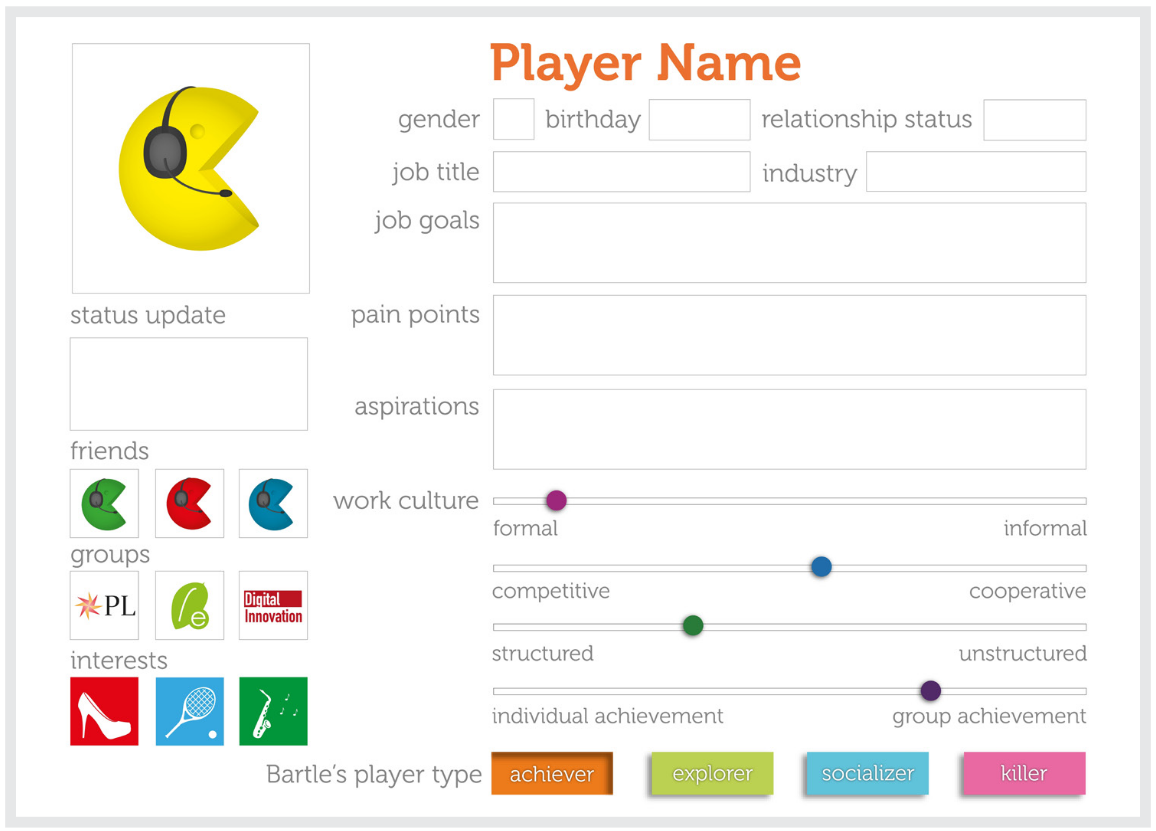
\includegraphics[width=0.8\textwidth]{Content/Theory/PlayerPersona.png}
		\caption{Player Persona Template}
		\cite[p. 46]{kumarGamificationWorkDesigning2013}
		\label{fig:playerPersonaTemplate}
	\end{figure}
	
	\item Mission \newline
	The main goal of the gamification process is identified, the so called mission. Figure \ref{fig:smartMission} represents the S.M.A.R.T Mission process to identify the mission. First of all, the current situation is analyzed and the target business outcome is studied. Based on the gained knowledge a mission for the gamification process is set. It should be specific, measurable, actionable, realistic and time-bound. \cite[p. 49-52]{kumarGamificationWorkDesigning2013}
	
	\begin{figure}[htbp] 
		\centering
		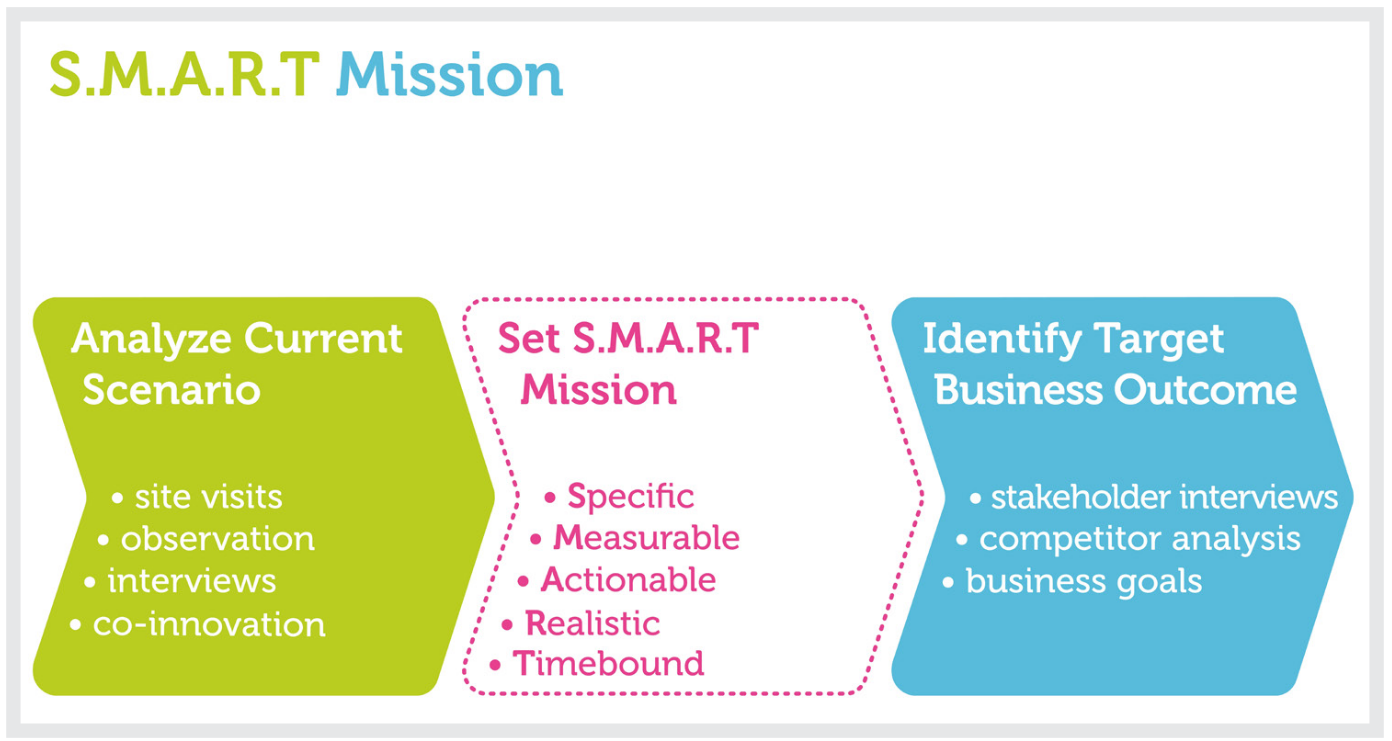
\includegraphics[width=1.0\textwidth]{Content/Theory/SmartMission.png}
		\caption{S.M.A.R.T. Mission}
		\cite[p. 50]{kumarGamificationWorkDesigning2013}
		\label{fig:smartMission}
	\end{figure}

	\item Human Motivation \newline
	Based on the theory behind human motivation (chapter \ref{sec:theoryBb}) the concrete motivational factors for the different user personas are defined. \cite[p. 59-67]{kumarGamificationWorkDesigning2013}
	
	\item Game Mechanics \newline
	Game mechanics represent the area of adding concrete gameful patterns to a non-game environment. As part of motivational design patterns gameful patterns are described in chapter \ref{GamefulPatterns}. While implementing gameful patterns in non game environments one should take into account that adding all patterns to an application normally doesn't reach the resumed aim. Hence, the selection of fitting patterns must be adapted to the prescribed context. The main aim behind adding gameful patterns is to build a positive engagement loop centering the user/player. Figure \ref{fig:engagementLoop} shows the four main steps of the engagement loop, starting with a motivating emotion.  \cite[p. 69-71]{kumarGamificationWorkDesigning2013}
	
	\begin{figure}[htbp] 
		\centering
		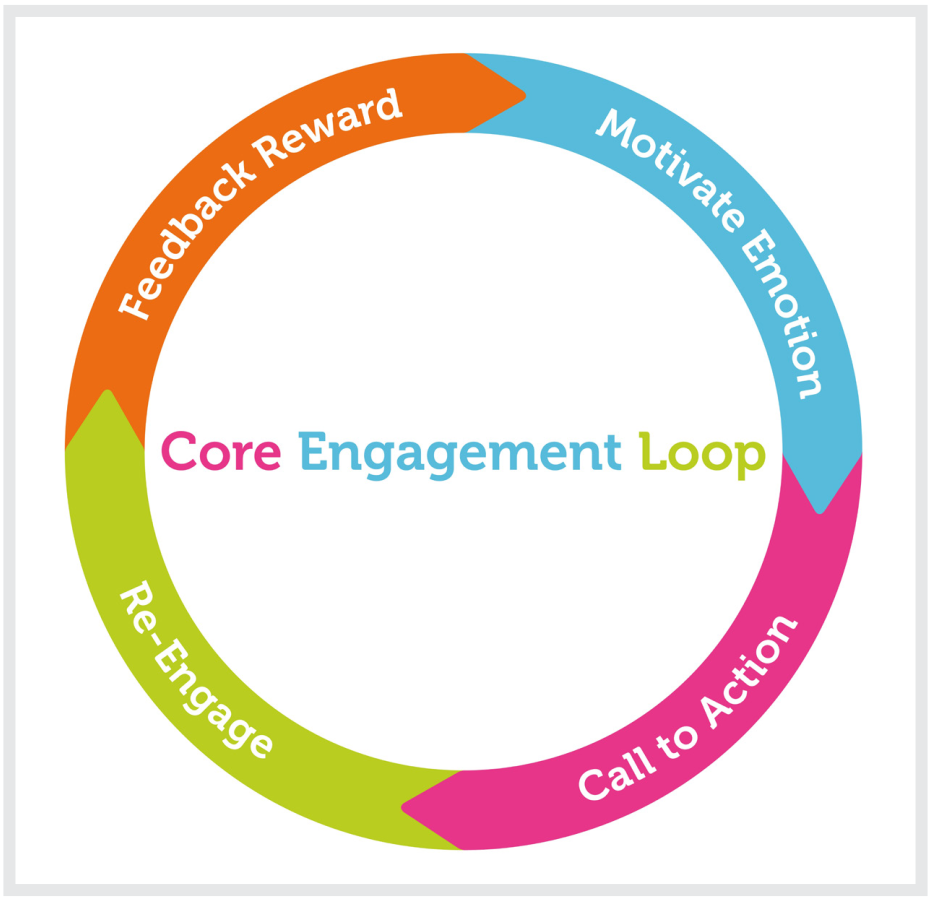
\includegraphics[width=0.5\textwidth]{Content/Theory/EngagementLoop.png}
		\caption{Engagement Loop}
		\cite[p. 88]{kumarGamificationWorkDesigning2013}
		\label{fig:engagementLoop}
	\end{figure}
	
	\item Manage, Monitor and Measure \newline
	After applying specific game mechanics to an application there are few points left, which should be observed in production. On one hand, the mission should be managed. Based on the S.M.A.R.T. Mission process the identified mission should be checked frequently and if needed adapted. On the other hand, the user/player behavior should be monitored and measured to evaluate the effectiveness of the implemented patterns. This can be done in a qualitative way by using surveys and interviews and in a quantitative manner by tracking and data evaluation. Based on the acquired knowledge the application can be enhanced in the future.	\cite[p. 92-96]{kumarGamificationWorkDesigning2013}
\end{enumerate}

\newpage

\subsection{Discussion}
\label{sec:theoryBe}

A literature review from Hamari, Koivisto and Sarsa \cite{hamariDoesGamificationWork2014} tries to answer the question if gamification works. Therefore quantitative and qualitative studies on this topic had been analyzed, resulting in the statement that quantitatively there are positive effects of gamification, but the gamification elements are only partly responsible for these effects. The analysis of qualitative studies resulted in the statement that gamification is more versatile than often assumed. \cite[p. 3029, 3030]{hamariDoesGamificationWork2014} 

The next question arising from this is: What are the reasons for these results and which disruptive factors harm the effectiveness of gamification? Therefore, the study's conclusions are analyzed resulting in two aspects: Influence of the gamified context and user qualities. \cite[p. 3029, 3030]{hamariDoesGamificationWork2014}

\paragraph*{Influence of the gamified context}

The context which should be gamified influences the prospects of success. Hamari, Koivisto and Sarsa name three contextual factors \cite[p. 3029, 3030]{hamariDoesGamificationWork2014}:
\begin{enumerate}
	\item Social environment: \newline
	In order to form behaviors  one key for success is the voluntary nature of doing something. \cite[p. 3030]{hamariDoesGamificationWork2014}
		
	\item Nature of the system: \newline
	Systems which should be gamified can be hedonic or utilitarian. Hedonic systems support their users reaching desire and pleasure. \cite[p. 3030]{hamariDoesGamificationWork2014}
	They are based on the philosophical concept of hedonism, which centers the human pursuit of desire and pleasure. Only the steady pursuit can reach intrinsically motivation. \cite[p. LV ]{mueller-saloHenrySidgwickUtilitarismus2019}
		
	On the contrary utilitarian systems are purpose-oriented. The underlying philosophical concept is called utilitarianism. It is based on the principle that an action is morally correct when it maximizes the aggregated overall benefit, that is the sum of the welfare of all concerned. \cite[p. 3 ]{mueller-saloHenrySidgwickUtilitarismus2019}
		
	\item Involvement of the user: \newline
	Depending on the application's context there are two types how a user can be involved: cognitive or affective. \cite[p. 3030]{hamariDoesGamificationWork2014} Cognitive involvement describes the user's interest respective an application. When being affectively involved, one evolves specific feelings towards the application. In the context of business application the user's are normally involved cognitively. \cite{zaichkowskyPersonalInvolvementInventory2013}
\end{enumerate}

%Korrumpierungseffekt
The overjustification effect describes the consequences how intrinsically motivated users change their behavior when extrinsic incentives are added. By adding extrinsic motivation the intrinsic motivation decreases. \cite[p. 9-13]{bierhoffeditorEnzyklopaediePsychologieSoziale2016}
	
Moreover there is the risk of false incentives. When applying gamification patterns without thoroughly thinking about the consequences it can lead to misguided behavior. For example, when every user who contributes a risk to the project gets points, that will create a false incentive, leading to lots of contributed risks, but little attention to the risk management of each risk. \cite[p.69]{kumarGamificationWorkDesigning2013}
 
\paragraph*{User qualities}

The different abilities and qualities of users have a decisive influence on the user's behavior while using the application and thus the success of gamification. Each user interacts differently with the application. For example, positive gamification effects where only measurable inside a specific context or with specific users. \cite[p. 3029, 3030]{hamariDoesGamificationWork2014}


\newpage
